% $Id: figures.tex 61168 2014-09-25 23:10:50Z roldeman $
% ===============================================================================
% Purpose: including figures in the standard template
% Author: Tomasz Skwarnicki, Ulrik Egede
% Created on: 2010-09-24
% ===============================================================================

\section{Figures}
\label{sec:Figures}

A standard \lhcb style file for use in production of figures in \root
is in the \urania package \texttt{RootTools/LHCbStyle} or directly in
\svn at
\texttt{svn+ssh://svn.cern.ch/reps/lhcb/Urania/trunk/RootTools/LHCbStyle}.
It is not mandatory to use this style, but it makes it easier to
follow the recommendations below. For labelling the axis and legends
it is recommended to use (as in the examples) the same text fonts as
in the main text. When using ROOT to produce the plots, use the
upright symbol font for text. The slanted font exists, but does not
look good. It is also possible to use consistently upright sans-serif
fonts for the text (slide style). However, styles should not be
mixed. For particle symbols, try to use the same font (roman/italic)
as is used in the text.

Pull plots are control plots, which are useful in analysis notes.  
Normally they are not shown in papers, unless one wants to emphasise 
regions where a fit does not describe the data. For satisfactory 
fits, in a paper it is sufficient to simply state the fact and/or
give the $\chisq/$ndf.


Figure~\ref{fig:example} shows an example of how to include an eps
or pdf figure with the \texttt{\textbackslash includegraphics} command
(eps figures will not work with \texttt{pdflatex}). Note that if the
graphics sits in \texttt{figs/myfig.pdf}, you can just write
\texttt{\textbackslash includegraphics\{myfig\}} as the \texttt{figs}
subdirectory is searched automatically and the extension \texttt{.pdf}
(\texttt{.eps}) is automatically added for \texttt{pdflatex}
(\texttt{latex}).
\begin{figure}[tb]
  \begin{center}
    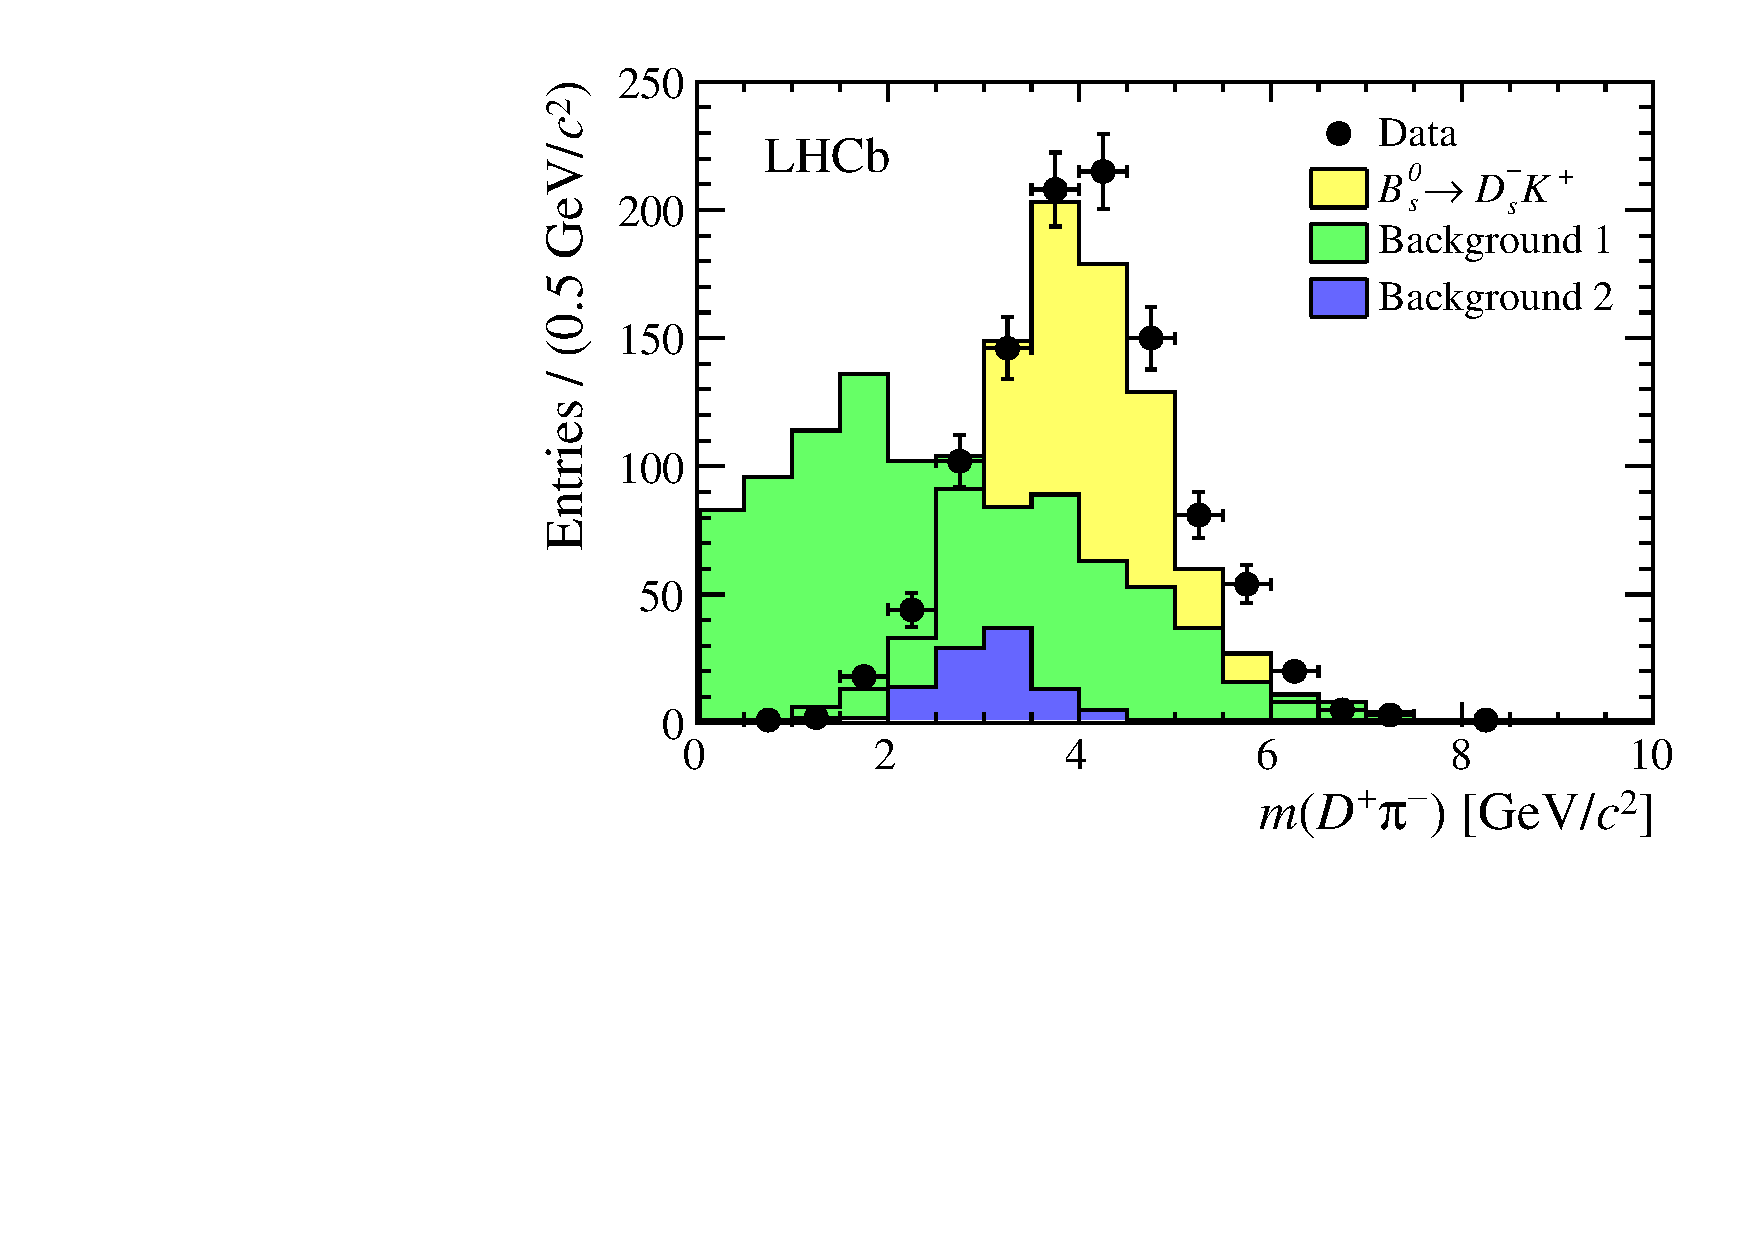
\includegraphics[width=0.49\linewidth]{Example1DPlot-python-1}\put(-32,133){(a)}
    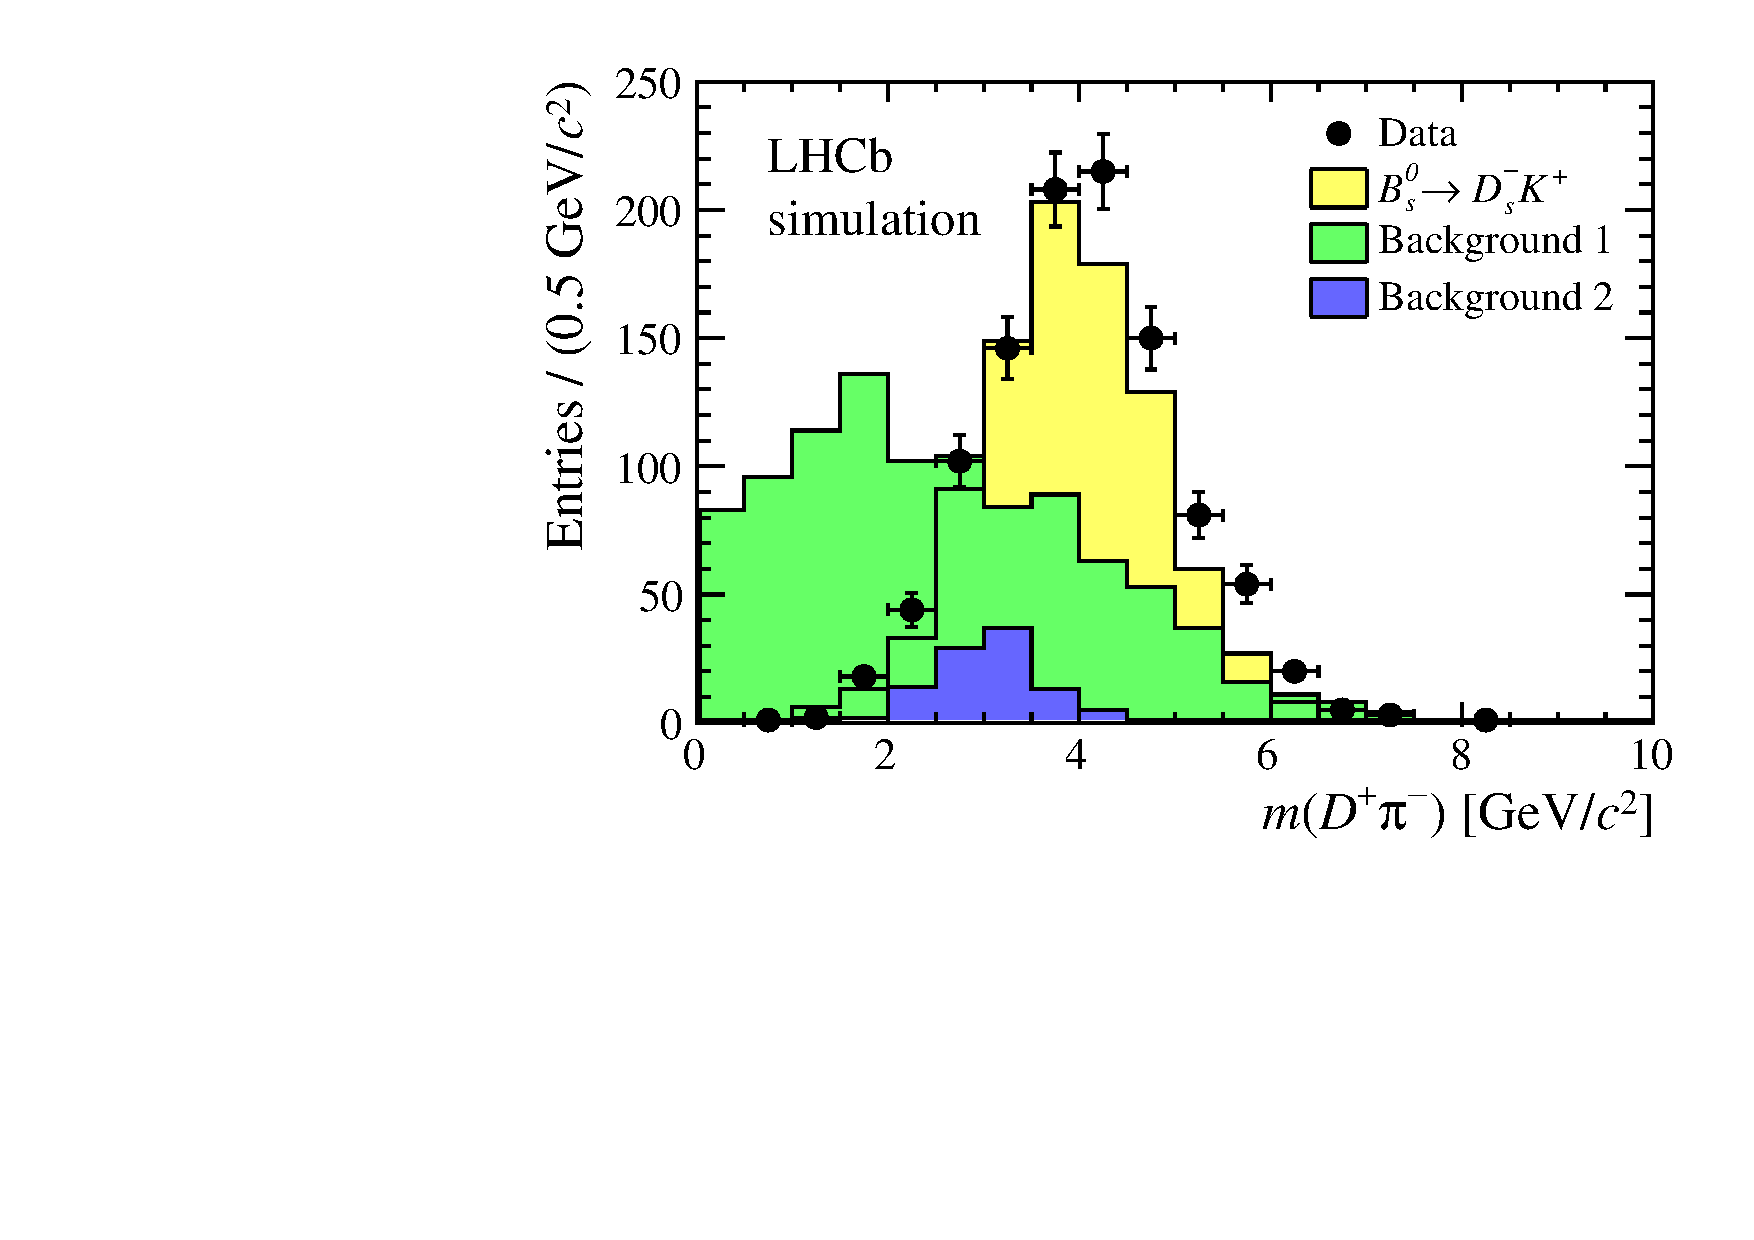
\includegraphics[width=0.49\linewidth]{Example1DPlot-python-1_sim}\put(-32,133){(b)}
    \vspace*{-0.5cm}
  \end{center}
  \caption{
    %\small %captions should be a little bit smaller than main text
    Example plots for (a) data and (b) simulation using the \lhcb style from the \urania package
    \texttt{RootTools/LHCbStyle}. The signal data is shown as points
    with the signal component as yellow (light shaded), background 1 as green
    (medium shaded) and background 2 as blue (dark shaded).}
  \label{fig:example}
\end{figure}

\begin{enumerate}

\item Figures should be legible at the size they will appear in the
  publication, with suitable line width.  Their axes should be
  labelled, and have suitable units (e.g. avoid a mass plot with
  labels in \mevcc if the region of interest covers a few \gevcc
  and all the numbers then run together).  Spurious background shading
  and boxes around text should be avoided.

\item For the $y$-axis, ``Entries'' or ``Candidates'' is approriate in case no
background subtraction has been applied. Otherwise ``Yield'' or ``Decays''
may be more appropriate. If the unit on the $y$-axis corresponds to 
the yield per bin, indicate so, for example ``Entries / (5\mevcc)'' or ``Entries per 5\mevcc''.


\item Fit curves should not obscure the data points, and
   data points are best (re)drawn over the fit curves. In this
   case avoid in the caption the term ``overlaid'' when
   referring to a fit curve, and instead use the words  
   ``shown'' or ``drawn''.

\item Colour may be used in figures, but the distinction between
  differently coloured areas or lines should be clear also when the
  document is printed in black and white, for example through
  differently dashed lines. The \lhcb style mentioned above implements
  a colour scheme that works well but individual adjustments might be
  required.

\item Using different hatching styles helps to disinguished filled areas, 
also in black and white prints. Hatching styles 3001-3025 should be
avoided since they behave unpredictably under zooming and scaling. 
Good styles for ``falling hatched'' and ``rising hatched'' are 3345 and 3354.


\item Figures with more than one part should have the parts labelled
  (a), (b) \etc, with a corresponding description in the caption;
  alternatively they should be clearly referred to by their position,
  e.g. Fig.~1\,(left). In the caption, the labels (a), (b) \etc should
  precede their description. When referencing specific sub-figures,
  use ``see Fig. 1(a)'' or ``see Figs. 2(b)-(e)''.

\item All figures containing \lhcb data should have \lhcb written on
  them. For preliminary
  results, that should be replaced by ``LHCb preliminary''.
  Figures that only have simulated data should display ``LHCb simulation''.
  Figures that do not depend on LHCb-specific software (\eg only on \pythia)
  should not have any label.


\end{enumerate}
